\documentclass[12pt,a4paper]{article}
\usepackage[left=2.00cm,right=2.00cm]{geometry}
\usepackage{graphicx}
\usepackage[T1]{fontenc}
\usepackage[utf8]{inputenc}
\usepackage{float}
\usepackage{multirow}
\usepackage{caption}
\usepackage{natbib}
\usepackage{graphicx}
\usepackage{longtable}
\usepackage{subcaption}
\usepackage{amsmath}
\usepackage[table,xcdraw]{xcolor}
\usepackage{siunitx}
\usepackage{hyperref}
\usepackage{placeins}
%to jest komenda do pisania jednostek w trybie matematycznym, \un{jednostka}, żeby jednostka nie była pochylona itp.
\newcommand{\un}[1]{\ensuremath{\ \mathrm{#1}}}

% ---- additions required by this document (see report) ----
\usepackage{amssymb}   % \mathbb, \lesssim, \gtrsim
\usepackage{booktabs}  % \toprule / \midrule / \bottomrule
\usepackage{listings}  % 21 fenced code blocks, with line breaking
\usepackage{pifont}    % the check / cross glyphs in the MLflow run table

\graphicspath{{figures/}}
\sisetup{group-minimum-digits=4}
\hypersetup{hidelinks}
\setlength{\emergencystretch}{3em}

\lstdefinestyle{readme}{%
  basicstyle=\ttfamily\small,
  breaklines=true,
  breakatwhitespace=false,
  postbreak=\mbox{\textcolor{gray}{$\hookrightarrow$}\space},
  columns=flexible,
  keepspaces=true,
  showstringspaces=false,
  keywordstyle={}, commentstyle={}, stringstyle={}, identifierstyle={},
  frame=single,
  rulecolor=\color{gray},
  framesep=4pt,
  xleftmargin=6pt,
  xrightmargin=2pt,
  aboveskip=1em, belowskip=1em,
  upquote=true,
}
\lstset{style=readme}

\title{NN-Adaptive Bayesian Quantum Estimation}
\author{Michal Chrzanowski}
\date{7 September 2026}

\begin{document}
\maketitle

\section{Introduction}\label{sec:introduction}
This report concerns learning \textbf{when to measure} a qubit, so that one learns \textbf{what its frequency is} as fast as physically possible.

The work implements adaptive Bayesian experimental design for single-qubit Ramsey frequency estimation. A sequential Monte Carlo filter maintains a posterior over the unknown Larmor frequency $\omega$; a policy reads that posterior and picks the interrogation time $t$ for the next shot; the measurement outcome sharpens the posterior; and the cycle repeats. The policy is trained either by reinforcement learning (TRPO) or by a gradient-free evolutionary search (CEM), following Fiderer, Schuff \& Braun, \emph{Neural-network heuristics for adaptive Bayesian quantum estimation}.

Equation numbers quoted throughout refer to the preprint (dated 2020-03-05); numbering may differ from the published version, PRX Quantum \textbf{2}, 020303 (2021). The physics has been checked against that preprint equation by equation. Where this implementation departs from the paper --- and it does, in ways that matter --- the departures are catalogued in \hyperref[sec:divergences-from-fiderer-et-al]{Divergences from Fiderer et al.}

\FloatBarrier
\section{Theory}\label{sec:theory}

\subsection{Physics Theory}\label{sec:physics-theory}

\subsubsection{The experiment}\label{sec:the-experiment}
The system is a single qubit undergoing \textbf{Ramsey interferometry} in the presence of pure dephasing:

\begin{enumerate}
  \item Prepare $|+\rangle = (|0\rangle + |1\rangle)/\sqrt{2}$.
  \item Let it precess freely under $H = \tfrac{\omega}{2}\sigma_z$ for a time $t$. This is the \textbf{control variable} --- the one thing the experimenter chooses.
  \item Apply a $\pi/2$ read-out pulse and measure in the computational basis.
  \item Record the binary outcome $d \in \{0, 1\}$.
\end{enumerate}
The qubit is not isolated: transverse noise destroys the coherence $\rho_{01}(t) = \rho_{01}(0)\,e^{-t/T_2}e^{-i\omega t}$ on a timescale $T_2$.

\subsubsection{The likelihood}\label{sec:the-likelihood}
Solving the Lindblad pure-dephasing master equation and applying the Born rule gives the outcome probability

\begin{align}
P(d=0 \mid \omega, t)
  &= e^{-t/T_2}\cos^{2}\!\left(\frac{\omega t}{2}\right) + \frac{1 - e^{-t/T_2}}{2} \nonumber \\
  &\equiv \frac{1}{2}\bigl[\, 1 + e^{-t/T_2}\cos(\omega t) \,\bigr],
\label{eq:likelihood}
\end{align}
and $P(d=1) = 1 - P(d=0)$. The two forms are algebraically identical.

The expression reads as a \textbf{decaying interference fringe}:

\begin{table}[H]
  \centering
  \caption{The likelihood.}
  \label{tab:the-likelihood}
  \small
  \begin{tabular}{ll}
  \toprule
  term & meaning \\
  \midrule
  $\cos^2(\omega t/2)$ & the Ramsey fringe --- this is what carries information about $\omega$ \\
  $v(t) = e^{-t/T_2}$ & the \textbf{visibility}, or coherent fraction \\
  $(1-v)/2$ & the fully dephased fraction, which returns a coin flip and tells you nothing \\
  \bottomrule
  \end{tabular}
\end{table}
As $t \to \infty$ the visibility vanishes, $P(d=0) \to 1/2$, and the measurement becomes pure noise. \textbf{Decoherence therefore imposes a hard ceiling on how long it is worth interrogating.}

Both the simulator and the filter's likelihood use this same expression, and $T_2$ is treated as exactly known. The model is well-specified: there is no model mismatch and no nuisance parameter.

\subsubsection{What is being estimated}\label{sec:what-is-being-estimated}
\begin{table}[H]
  \centering
  \caption{What is being estimated.}
  \label{tab:what-is-being-estimated}
  \footnotesize
  \begin{tabular}{>{\raggedright\arraybackslash}p{0.124\linewidth}>{\raggedright\arraybackslash}p{0.438\linewidth}>{\raggedright\arraybackslash}p{0.344\linewidth}}
  \toprule
  quantity & value & where \\
  \midrule
  parameter & $\omega$, a single scalar (the Larmor frequency / detuning) & \texttt{seq\_\allowbreak{}montecarlo.\allowbreak{}py:\allowbreak{}9} \\
  prior & $\omega \sim \mathrm{Uniform}(0, 1)$, so $\mathrm{Var}[\omega] = 1/12 \approx 0.0833$ & \texttt{seq\_\allowbreak{}montecarlo.\allowbreak{}py:\allowbreak{}9}, \texttt{:\allowbreak{}127} \\
  true values & drawn from the same $\mathrm{Uniform}(0,1)$ & \texttt{train\_\allowbreak{}TRPO\_\allowbreak{}baseline.\allowbreak{}py:\allowbreak{}67} \\
  coherence time & $T_2 = 10$ & \texttt{modules/\allowbreak{}simulation.\allowbreak{}py:\allowbreak{}31} \\
  control & $t \in [0.1,\ 3000]$ & \texttt{train\_\allowbreak{}TRPO\_\allowbreak{}baseline.\allowbreak{}py:\allowbreak{}54-\allowbreak{}55} \\
  \bottomrule
  \end{tabular}
\end{table}
Units are arbitrary --- $\omega$ and $t$ only ever appear as the product $\omega t$, and $T_2$ shares the units of $t$. With $\omega \lesssim 1$ and $T_2 = 10$, roughly $\omega T_2 \lesssim 10$ radians of phase accumulate before coherence is lost, so a few fringes are resolvable within the coherence window.

\subsubsection{Why long interrogation times stop helping}\label{sec:aside-why-long-interrogation-times-stop-helping}
This argument is not part of the paper's framework; it is included because it explains the shape of the results. Differentiating the likelihood gives the single-shot Fisher information

\begin{equation}
I(\omega; t) = \frac{(\partial_\omega p_0)^{2}}{p_0(1-p_0)}
             = \frac{t^{2} v^{2} \sin^{2}(\omega t)}{1 - v^{2}\cos^{2}(\omega t)},
\qquad v = e^{-t/T_2}.
\label{eq:fisher}
\end{equation}
Without decoherence ($v \to 1$) this is just $I = t^2$: information grows quadratically in interrogation time, which is why longer is better and why adaptive schemes that grow $t$ pay off. With finite $T_2$ the envelope $t^2 e^{-2t/T_2}$ peaks at $t = T_2$, so information per shot is \textbf{bounded} at $I_{\max} \approx 0.135\,T_2^2$. Numerically, for $T_2 = 10$ the optimum sits at $t^\star \approx 8.4$--$9.5$ depending on $\omega$.

This matches the paper's observation that ``times which exceed $T_2$ tend to yield no information, which explains why the Bayes risk saturates for the exp-sparse heuristic.''

\subsubsection{The competing constraint: phase ambiguity}\label{sec:the-competing-constraint-phase-ambiguity}
Fisher information is a \emph{local} quantity, and maximising it is the wrong move while the prior is still broad. The likelihood depends on $\omega$ only through $\cos(\omega t)$, which is periodic. Over the prior support $\Delta\omega = 1$ the fringe wraps once $t > 2\pi \approx 6.28$: several well-separated $\omega$ then produce the same phase, the posterior goes \textbf{multimodal}, and the filter cannot resolve the aliases.

A good policy must therefore trade off:

\begin{itemize}
  \item \textbf{small $t$} --- unambiguous, but low information per shot ($I \sim t^2$);
  \item \textbf{$t \approx T_2$} --- maximum information per shot, but aliases a broad prior;
  \item \textbf{$t \gg T_2$} --- decohered, zero information, strictly wasted.
\end{itemize}
The resolution is to grow $t$ \emph{as the posterior narrows}, keeping the phase spread across the posterior at roughly one radian --- exactly what the $\sigma^{-1}$ and PGH heuristics do, and what an RL policy is expected to discover.

Because those heuristics only reach large $t$ \emph{after} the posterior has collapsed, they never alias, which is why the paper discusses large-$t$ failure purely in terms of decoherence. A \textbf{constant} $t = 10$, by contrast, aliases from the very first shot --- which is why it performs so badly in the \hyperref[sec:baseline-results]{measured results} despite sitting at the Fisher optimum. The two statements are consistent; they describe different situations.

\FloatBarrier
\subsection{Algorithmic Theory}\label{sec:algorithmic-theory}

\subsubsection{The figure of merit: Bayes risk}\label{sec:the-figure-of-merit-bayes-risk}
This is a \textbf{Bayesian} estimation problem, and the quantity everything is judged by is the \textbf{Bayes risk} --- Fiderer Eq. (1):

\begin{equation}
r\bigl(h \mid p(\theta)\bigr) = \mathbb{E}_{D_k}\bigl[\, \mathrm{tr}\,\mathrm{Cov}(\theta \mid D_k) \,\bigr],
\label{eq:bayes-risk}
\end{equation}
where $h$ is the experiment-design heuristic, $D_k = (d_1,\dots,d_k)$ the measurement record, and smaller is better. It is the risk of the quadratic loss $L(\hat\theta_k, \theta) = \lVert\hat\theta_k - \theta\rVert_2^2$ under the Bayes estimator $\hat\theta_k(D_k) = \mathbb{E}[\theta \mid D_k]$ --- that is, the posterior mean, which is exactly what this implementation reports as \texttt{posterior\_\allowbreak{}mean}.

For the single-parameter, experiment-limited case implemented here, the trace is over a $1\times1$ covariance and the expectation is estimated by averaging over true $\omega$ values. \textbf{So the Bayes risk is precisely the mean final posterior variance} reported as \texttt{final\_\allowbreak{}variance\_\allowbreak{}mean}, by which the \hyperref[sec:baseline-results]{baseline results} rank the methods. They are the same number; the paper's name for it is the Bayes risk.

Note the framing: the paper is explicit that the \emph{frequentist} route to experiment design goes ``with the Cram\'er--Rao bound formalism by maximizing the quantum Fisher information'', and it deliberately takes the Bayesian route instead. Fisher information is a useful sanity check here (\hyperref[sec:aside-why-long-interrogation-times-stop-helping]{above}) but it is \textbf{not} the objective.

\subsubsection{The reward}\label{sec:the-reward}
The reward is the \textbf{reduction in traced posterior covariance} at each step --- Fiderer Eq. (2):

\begin{align}
R(D_k) &= \mathrm{tr}\,\mathrm{Cov}(\theta \mid D_{k-1}) - \mathrm{tr}\,\mathrm{Cov}(\theta \mid D_k) \nonumber \\
       &\xrightarrow{\ d=1\ } V_{k-1} - V_k,
\label{eq:reward}
\end{align}
with $V_k = \sum_i w_i(\omega_i - \bar\omega)^2$. This is not an arbitrary choice, and it is \textbf{not} a weaker substitute for an information-gain reward. The paper's reasoning: the negative Bayes risk is the obvious reward but is far too slow to compute inside a training loop, whereas Eq. (2) is cheap in the SMC framework \emph{and} telescopes to it. Eq. (3), for $N$ experiments per episode:

\begin{equation}
\mathbb{E}_{D_N}\left[\sum_{j=1}^{N} R(D_j)\right] = \mathrm{const} - r\bigl(h \mid p(\theta)\bigr),
\qquad \mathrm{const} = \mathrm{tr}\,\mathrm{Cov}(\theta).
\label{eq:telescope}
\end{equation}
So maximising the episode return \textbf{provably minimises the Bayes risk} --- but the identity holds only for an \emph{undiscounted} return. The paper states this explicitly: ``RL has the goal to maximize the expected discounted reward which equals the left-hand side of Eq. (3) \textbf{because we set the discount factor to one}.'' This implementation sets $\gamma = 0.99$, which breaks it --- see \hyperref[sec:4-gamma--099-breaks-the-bayes-risk-identity]{the discussion of the discount factor}.

\subsubsection{The inference layer: SMC particle filter}\label{sec:the-inference-layer-smc-particle-filter}
$\omega$ is a \textbf{static} parameter --- it does not evolve --- so the filter only ever reweights particles; the particle locations move solely during resampling.

\textbf{Representation.} $N$ particles $\{\omega_i\}$ with log-weights $\{\log w_i\}$. Shapes are \texttt{(N, 1)} / \texttt{(N,)} in the NumPy path, \texttt{(B, N, 1)} / \texttt{(B, N)} in the batched Torch path, where \texttt{B} indexes independent experiments.

\textbf{Bayes update.} Log-domain throughout:

\begin{equation}
\log w_i \leftarrow \log w_i + \log P(d \mid \omega_i, t) - \mathrm{logsumexp}(\cdot).
\label{eq:bayes-update}
\end{equation}
Renormalised every step, so weights always sum to one.

\textbf{Effective sample size.} The Kish ESS, $\mathrm{ESS} = 1/\sum_i w_i^2 \in [1, N]$.

\textbf{Resampling} fires when $\mathrm{ESS} < 0.75N$ --- an aggressive threshold (0.5N is the usual default), so it triggers on most steps. Two schemes exist; the default everywhere is \textbf{Liu--West kernel resampling} ($a = 0.98$):

\begin{equation}
\omega_i' = a\,\omega_{\mathrm{idx}(i)} + (1-a)\,\bar{\omega} + \varepsilon_i,
\qquad \varepsilon_i \sim \mathcal{N}\bigl(0,\, h^{2}\Sigma\bigr), \quad h^{2} = 1 - a^{2}.
\label{eq:liu-west}
\end{equation}
The shrinkage toward the weighted mean exactly cancels the variance added by the jitter ($a^2\Sigma + h^2\Sigma = \Sigma$), so the posterior's first two moments are preserved. The jitter is what prevents particle impoverishment --- plain multinomial resampling would collapse all particles onto a handful of duplicated values, since a static parameter never gets diffused by process noise.

\subsubsection{The control problem}\label{sec:the-control-problem}
The control problem is framed as a Gymnasium environment, \texttt{AdaptiveSMCEnv}:

\begin{table}[H]
  \centering
  \caption{The control problem.}
  \label{tab:the-control-problem}
  \scriptsize
  \begin{tabular}{ll}
  \toprule
  \textbf{observation} & \texttt{[posterior\_\allowbreak{}mean, posterior\_\allowbreak{}var, *last\_\allowbreak{}30\_\allowbreak{}interrogation\_\allowbreak{}times]} $\rightarrow$ \texttt{Box(32,)} \\
  \textbf{action} & interrogation time $t$ $\rightarrow$ \texttt{Box(0.\allowbreak{}1, 3000.\allowbreak{}0, (1,))} \\
  \textbf{reward} & $V_{k-1} - V_k$ \\
  \textbf{episode} & 100 measurements (training) / 125 (evaluation), one true $\omega$ per episode \\
  \bottomrule
  \end{tabular}
\end{table}

\subsubsection{Methods implemented}\label{sec:methods-implemented}
Two learned policies are implemented:

\begin{table}[H]
  \centering
  \caption{Learned policies.}
  \label{tab:learned-policies}
  \footnotesize
  \begin{tabular}{>{\raggedright\arraybackslash}p{0.062\linewidth}>{\raggedright\arraybackslash}p{0.257\linewidth}>{\raggedright\arraybackslash}p{0.357\linewidth}>{\raggedright\arraybackslash}p{0.205\linewidth}}
  \toprule
  method & optimiser & network & entry point \\
  \midrule
  \textbf{TRPO} & trust-region policy optimisation (\texttt{sb3\_\allowbreak{}contrib}) & \texttt{MlpPolicy}, $\pi$ and $V$ both \texttt{[256, 256]} & \texttt{pipeline/\allowbreak{}train\_\allowbreak{}TRPO\_\allowbreak{}baseline.\allowbreak{}py} \\
  \textbf{CEM} & cross-entropy method over the flat 545-dim weight vector & \texttt{TimePolicy\_\allowbreak{}Fiderer\_\allowbreak{}16} --- one hidden layer of 16, \texttt{Tanh}, sigmoid-squashed output & \texttt{pipeline/\allowbreak{}train\_\allowbreak{}CEM.\allowbreak{}py} \\
  \bottomrule
  \end{tabular}
\end{table}
The CEM network squashes its output structurally, $t = t_{\min} + (t_{\max}-t_{\min})\,\sigma(z)$, so it can never emit an out-of-range time. The TRPO actor is an unbounded Gaussian whose sample is clipped in the environment step.

Alongside them sit six training-free baselines, which exist so the learned policies can be measured against something. All share one batched interface:

\begin{table}[H]
  \centering
  \caption{Training-free baselines.}
  \label{tab:training-free-baselines}
  \footnotesize
  \begin{tabular}{>{\raggedright\arraybackslash}p{0.307\linewidth}>{\raggedright\arraybackslash}p{0.254\linewidth}>{\raggedright\arraybackslash}p{0.345\linewidth}}
  \toprule
  policy & rule & why it's here \\
  \midrule
  \texttt{PGHPolicy} & $t = 1/\lvert\omega_1 - \omega_2\rvert$, two particles drawn from the posterior & the standard baseline in this literature (Wiebe \& Granade); keeps phase spread $\approx 1$ rad \\
  \texttt{PGHPolicy(t\_\allowbreak{}cap=T2)} & as above, capped at the coherence time & the standard fix for the decoherence-limited case \\
  \texttt{SigmaInversePolicy} & $t = k/\sigma$ & deterministic cousin of PGH, no sampling jitter \\
  \texttt{FixedTPolicy} & constant $t$ & non-adaptive control --- separates ``adaptivity helps'' from ``a good $t$ helps'' \\
  \texttt{ExponentialSweepPolicy} & $t_k = t_0 r^k$ & open-loop ladder; depends on step index, not on data \\
  \texttt{RandomTPolicy} & $t \sim U(0.1, 3000)$ & the do-nothing floor \\
  \bottomrule
  \end{tabular}
\end{table}

\FloatBarrier
\section{Training}\label{sec:training}
\textbf{TRPO.} Training runs for $10^5$ episodes of 100 steps --- $10^7$ timesteps --- with \num{10000} particles, both the policy and value networks of shape \texttt{[256, 256]}, and \texttt{target\_\allowbreak{}kl} $= 10^{-2}$. A full run takes \textbf{4--25 hours} on CPU. The spread is real rather than an estimate: the 100k-timestep run took 154\,s, while the 100M-timestep run averaged 6$\times$ slower per step. Checkpoints are written every \num{50000} timesteps, so a partially trained policy can be evaluated at any point and a crash costs at most one interval.

TRPO is trained \textbf{from scratch}. The paper's imitation-pretraining stage is not implemented; the consequences are taken up in \hyperref[sec:no-imitation-pretraining--the-leading-hypothesis-for-the-gap]{the discussion of divergences}.

\textbf{CEM.} Training runs for 100 generations at population 1000, elite fraction 0.1, with 2000 particles and 100-step episodes, optimising the flat 545-dimensional weight vector of \texttt{TimePolicy\_\allowbreak{}Fiderer\_\allowbreak{}16}. This takes \textbf{about 45 minutes} on CPU, roughly 27\,s per generation.

\textbf{Logging.} Logged per episode (TRPO) or per generation (CEM): \texttt{mean\_\allowbreak{}reward}, \texttt{mean\_\allowbreak{}init\_\allowbreak{}var}, \texttt{mean\_\allowbreak{}final\_\allowbreak{}var}, \texttt{mean\_\allowbreak{}ess}, \texttt{mean\_\allowbreak{}t}, \texttt{true\_\allowbreak{}omega}, plus \texttt{max\_\allowbreak{}reward}, \texttt{sigma\_\allowbreak{}mean} and \texttt{mu\_\allowbreak{}norm} for CEM. Parameters capture the full hyperparameter set alongside the git commit, branch and dirty flag.

The training runs on record are:

\begin{table}[H]
  \centering
  \caption{Experiment tracking.}
  \label{tab:experiment-tracking}
  \scriptsize
  \begin{tabular}{lllll}
  \toprule
  run & experiment & episodes logged & best \texttt{mean\_\allowbreak{}final\_\allowbreak{}var} & weights on disk \\
  \midrule
  \texttt{16eda430\ldots{}} & trpo\_baseline & \num{270764} & \textbf{9.28e-4} & \ding{55} crashed before saving \\
  \texttt{caaabcb8\ldots{}} & trpo\_baseline & \num{1003} & 2.85e-3 & \ding{51} \texttt{artifacts/\allowbreak{}trpo\_\allowbreak{}sb3\_\allowbreak{}policy.\allowbreak{}zip} \\
  \texttt{809c8bf6\ldots{}} & trpo\_baseline & 100 & 2.44e-3 & \ding{51} in \texttt{mlruns/\allowbreak{}3/\allowbreak{}} \\
  \texttt{b28a7dbc\ldots{}} & trpo\_baseline & 102 & 8.19e-2 & \ding{51} in \texttt{mlruns/\allowbreak{}3/\allowbreak{}} (barely learned) \\
  \texttt{bc96386c\ldots{}} & cem & 2 generations & --- & \ding{51} \texttt{mlruns/\allowbreak{}1/\allowbreak{}models/\allowbreak{}\ldots{}/\allowbreak{}model.\allowbreak{}pth} (untrained) \\
  \bottomrule
  \end{tabular}
\end{table}
The best training metric belongs to a run whose weights were lost; that episode is discussed in \hyperref[sec:7-the-best-result-in-the-repo-is-unreproducible]{the analysis below}. The archived CEM checkpoint is from a 2-generation run and is effectively untrained, so it supports no conclusion about CEM; the CEM results reported here come from the retrained network instead.

\FloatBarrier
\section{Evaluation}\label{sec:evaluation}
Two evaluation harnesses are used, and the distinction between them matters for how the numbers should be read.

\textbf{The paired comparison.} Every method is run through identical SMC and measurement code, which is what makes the numbers comparable at all: \textbf{2048 true $\omega$, 125 measurements, 2000 particles, seed 42, $T_2 = 10$}, with the same $\omega$ list for every method, so the comparison is paired and can be resolved per frequency. The prior variance is $1/12 = 0.0833$. For this single-parameter, experiment-limited problem the traced posterior covariance averaged over true $\omega$ is exactly the final posterior variance, so the reported final-variance columns are the \textbf{Bayes risk} of \hyperref[sec:the-figure-of-merit-bayes-risk]{Eq. (1)}. Lower is better.

\textbf{The reference harness.} A second path evaluates one $\omega$ at a time in NumPy at float64 and is the \textbf{reference implementation}: \num{10000} true $\omega$, 125 measurements, 2000 particles, Liu--West resampling. Its $\omega$ draw is independent of the training draw, so these are genuinely held-out frequencies. Where the two harnesses disagree, the reference path is the one to trust --- see \hyperref[sec:a-caveat-on-the-earlier-baseline-table]{the caveat on the batched harness}.

A GPU is not required for either. The batched rollout costs roughly 4.4\,ms per 125-step, 2000-particle episode on CPU, so a full \num{10000}-$\omega$ evaluation takes about a minute.

\FloatBarrier
\section{Analysis of Output Data}\label{sec:analysis-of-output-data}

\subsection{Baseline results}\label{sec:baseline-results}
\begin{center}
\footnotesize
\begin{longtable}{lllllll}
\caption{Baseline results.}\label{tab:baseline-results}\\
\toprule
method & median final var & mean & p10 & p90 & median $t$ & max $t$ \\
\midrule
\endfirsthead
\caption[]{Baseline results.\ (continued)}\\
\toprule
method & median final var & mean & p10 & p90 & median $t$ & max $t$ \\
\midrule
\endhead
\bottomrule
\endfoot
\textbf{fixed $t = 0.5$} & \textbf{4.09e-04} & 4.30e-04 & 3.05e-04 & 5.80e-04 & 0.50 & 0.5 \\
\textbf{fixed $t = 1$} & \textbf{4.33e-04} & 4.59e-04 & 2.98e-04 & 6.56e-04 & 1.00 & 1.0 \\
exponential sweep ($0.1 \cdot 1.05^k$) & 1.75e-03 & 2.04e-03 & 1.06e-03 & 3.24e-03 & 2.06 & 42.4 \\
\textbf{TRPO (learned)} & \textbf{2.03e-03} & 2.79e-03 & 9.26e-04 & 5.48e-03 & 0.75 & 4.1 \\
PGH (capped at 2) & 2.03e-03 & 2.04e-03 & 9.41e-04 & 3.09e-03 & 2.00 & 2.0 \\
fixed $t = 2$ & 2.06e-03 & 2.07e-03 & 9.74e-04 & 3.10e-03 & 2.00 & 2.0 \\
PGH (capped at $T_2$) & 3.72e-03 & 8.39e-03 & 1.44e-03 & 1.98e-02 & 10.00 & 10.0 \\
PGH (uncapped) & 5.19e-03 & 8.63e-03 & 2.46e-03 & 1.61e-02 & 11.44 & 3000.0 \\
$1/\sigma$ & 8.86e-03 & 1.31e-02 & 2.99e-03 & 2.92e-02 & 8.85 & 26.3 \\
fixed $t = 10$ & 8.02e-02 & 8.08e-02 & 6.76e-02 & 9.48e-02 & 10.00 & 10.0 \\
random $t \sim U(0.1, 3000)$ & 8.29e-02 & 8.07e-02 & 6.28e-02 & 8.71e-02 & 1502 & 3000.0 \\
\end{longtable}
\end{center}

\subsubsection{The learned policy loses to a constant}\label{sec:what-this-says}
TRPO lands mid-table at 2.03e-03 while a constant $t = 1$ reaches 4.33e-04. Because every method saw the identical $\omega$ list, the comparison can be made per-$\omega$: \textbf{fixed $t = 1$ beats TRPO on 99.85\% of the 2048 frequencies.} This is not sampling noise. TRPO also has by far the widest spread of any adaptive method (p10 9.26e-04 to p90 5.48e-03), which is the signature of an unstable policy rather than a merely suboptimal one --- \textbf{35.6\% of its actions sit exactly on the $t = 0.1$ floor}, in consecutive stretches with a median length of 22 measurements, visible as flat runs in the chosen-time traces.

Note this is the best \emph{loadable} checkpoint, from a 1000-episode run. The 68-hour run reached a 3$\times$ better training metric but its weights were lost, so this comparison cannot speak for a fully trained policy.

\subsubsection{Large $t$ is catastrophic, and that part is well understood}\label{sec:large-t-is-catastrophic}
Constant $t = 10$ (8.02e-02) barely improves on the prior (0.0833) despite sitting exactly at the Fisher-information optimum $t = T_2$. The reason is phase ambiguity: the likelihood depends on $\omega$ only through $\cos(\omega t)$, and over the prior support $\Delta\omega = 1$ the fringe wraps once $t > 2\pi \approx 6.28$. Every measurement is then consistent with several well-separated $\omega$, the posterior goes multimodal, and the filter cannot resolve it. \textbf{Maximising single-shot Fisher information is exactly the wrong objective while the prior is broad} --- which is precisely the tension the \hyperref[sec:the-competing-constraint-phase-ambiguity]{physics section} describes, and the reason PGH and $1/\sigma$, which both drive $t$ into the aliasing regime, do poorly here.

\subsubsection{Adaptivity buys nothing in this configuration}\label{sec:adaptivity-buys-nothing}
The best strategies are the two that never adapt at all, which is itself suspicious. After 125 shots at $t = 1$ the posterior has $\sigma \approx 0.021$, so the aliasing-safe bound has risen to $t < 2\pi/\sigma \approx 300$ --- an adaptive schedule \emph{should} be able to exploit that and beat any constant by a wide margin. None does. That points at the setup rather than at adaptivity: the reward goes numerically dead after $\sim$20 measurements, so there is almost no gradient signal for the late-episode behaviour where growing $t$ would pay off.

One caveat on the fine ordering: $t = 0.5$ edging out $t = 1$, and both beating $t = 2$, is \emph{not} explained by aliasing --- all three are well inside the unambiguous regime. Liu--West jitter and the aggressive $0.75N$ resample trigger are the likely culprits, but this has not been isolated.

\FloatBarrier
\subsection{Validation over \texorpdfstring{\num{10000}}{10 000} \texorpdfstring{$\omega$}{omega}}\label{sec:validation-over-10-000-omega-the-n-scripts}
Both retrained networks were evaluated on the NumPy reference harness over \num{10000} held-out frequencies.

\begin{table}[H]
  \centering
  \caption{Validation over \num{10000} $\omega$ (the N-scripts).}
  \label{tab:validation-over-10-000-omega-the-n-scripts}
  \scriptsize
  \begin{tabular}{lll}
  \toprule
   & TRPO & CEM \\
  \midrule
  training & \num{100002} episodes, $10^7$ timesteps, 2 h 24 m & 99 generations $\times$ 1000 pop, 54 min \\
  MLflow run & \texttt{4719c711} (exp 5) & \texttt{bf4ad6ae} (exp 4) \\
  \textbf{Bayes risk over \num{10000} $\omega$} & \textbf{2.173e-03} & \textbf{2.137e-03} \\
  mean $t$ & 4.00 & 6.67 \\
  min / max $t$ & 0.10 / 9.85 & 2.16 / 15.60 \\
  final ESS (of 2000) & 1960 & 1904 \\
  \bottomrule
  \end{tabular}
\end{table}
The two methods land in a \textbf{statistical tie} (2.17e-03 vs 2.14e-03, a 2\% difference) despite completely different optimisers and very different chosen times --- CEM settles on interrogation times roughly 1.7$\times$ longer than TRPO's, and never goes below $t = 2.16$, where TRPO ranges down to the action floor.

\subsubsection{Posterior collapse}\label{sec:posterior-collapse}
Mean posterior variance across all \num{10000} $\omega$, log scale. Both fall about 1.6 decades from the prior's 0.0833 and flatten out well before the 125th measurement --- the information-starved regime described above.

\begin{figure}[H]
  \centering
  \begin{subfigure}[t]{0.48\textwidth}
    \centering
    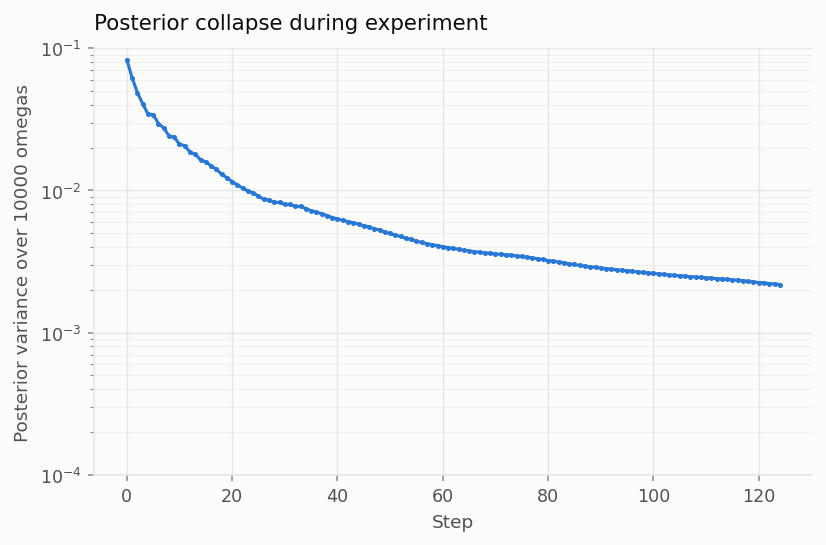
\includegraphics[width=\textwidth]{trpo_posterior_variance_over_omega_log}
    \caption{TRPO}
    \label{fig:posterior-collapse-trpo}
  \end{subfigure}\hfill
  \begin{subfigure}[t]{0.48\textwidth}
    \centering
    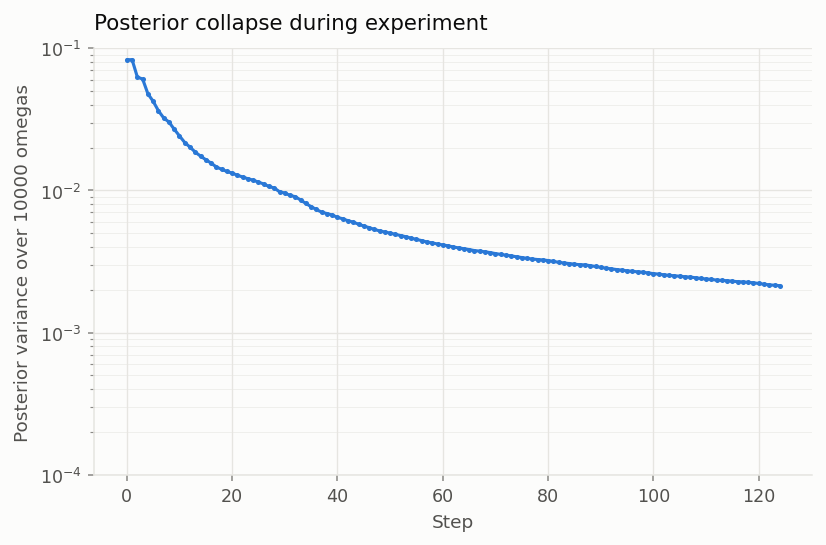
\includegraphics[width=\textwidth]{cem_posterior_variance_over_omega_log}
    \caption{CEM}
    \label{fig:posterior-collapse-cem}
  \end{subfigure}
  \caption{Posterior collapse.}
  \label{fig:posterior-collapse}
\end{figure}

\subsubsection{Chosen interrogation time}\label{sec:chosen-interrogation-time}
A single representative episode. This is where the two methods differ most.

\begin{figure}[H]
  \centering
  \begin{subfigure}[t]{0.48\textwidth}
    \centering
    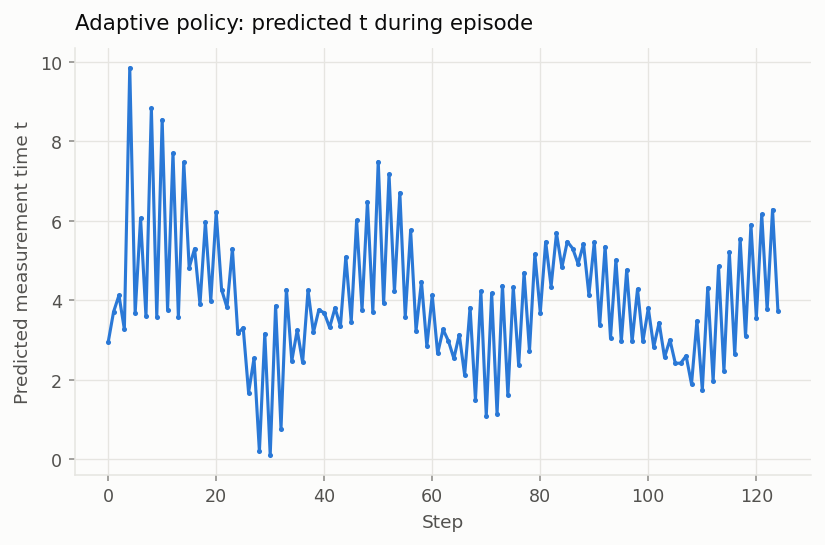
\includegraphics[width=\textwidth]{trpo_predicted_t}
    \caption{TRPO}
    \label{fig:chosen-interrogation-time-trpo}
  \end{subfigure}\hfill
  \begin{subfigure}[t]{0.48\textwidth}
    \centering
    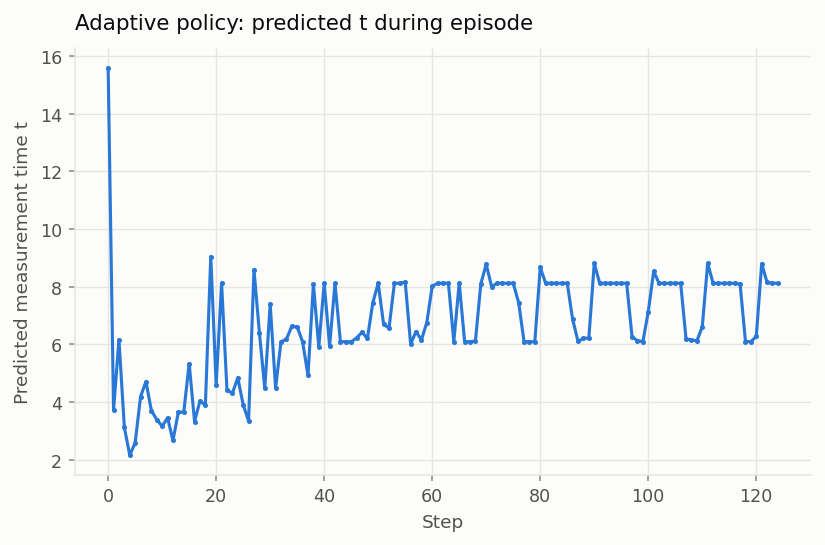
\includegraphics[width=\textwidth]{cem_predicted_t}
    \caption{CEM}
    \label{fig:chosen-interrogation-time-cem}
  \end{subfigure}
  \caption{Chosen interrogation time.}
  \label{fig:chosen-interrogation-time}
\end{figure}
TRPO oscillates hard between roughly 1 and 7, spiking to $\sim$10 in the opening measurements and never settling. CEM is smoother and biased higher. Neither shows the monotone growth in $t$ that the $\sigma^{-1}$/PGH analysis says an optimal adaptive policy should produce as the posterior narrows --- both are essentially oscillating around a fixed operating point, which is consistent with the constant-$t$ baselines being hard to beat.

Note that both spend time above $t = 2\pi \approx 6.28$, where the fringe aliases over the prior support. That is safe once the posterior is narrow, but TRPO's early spike to $t \approx 10$ happens while the posterior is still wide.

\subsubsection{Effective sample size}\label{sec:effective-sample-size}
\begin{figure}[H]
  \centering
  \begin{subfigure}[t]{0.48\textwidth}
    \centering
    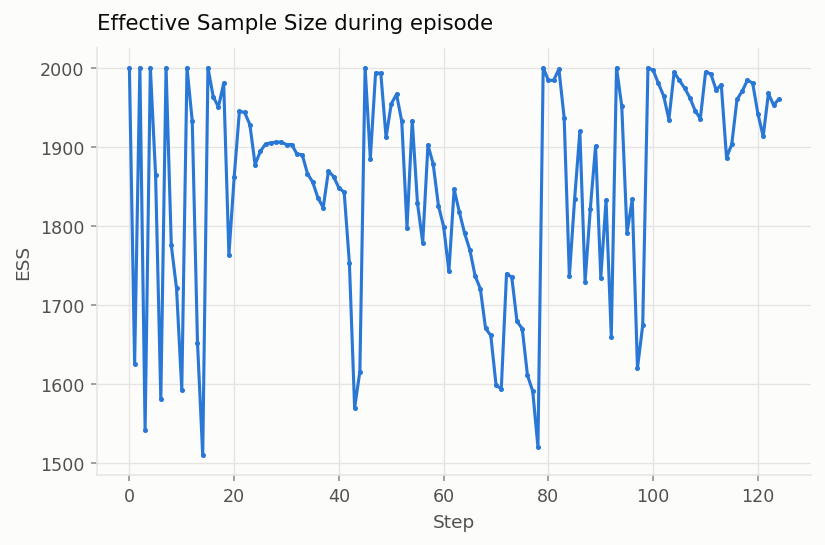
\includegraphics[width=\textwidth]{trpo_ess}
    \caption{TRPO}
    \label{fig:effective-sample-size-trpo}
  \end{subfigure}\hfill
  \begin{subfigure}[t]{0.48\textwidth}
    \centering
    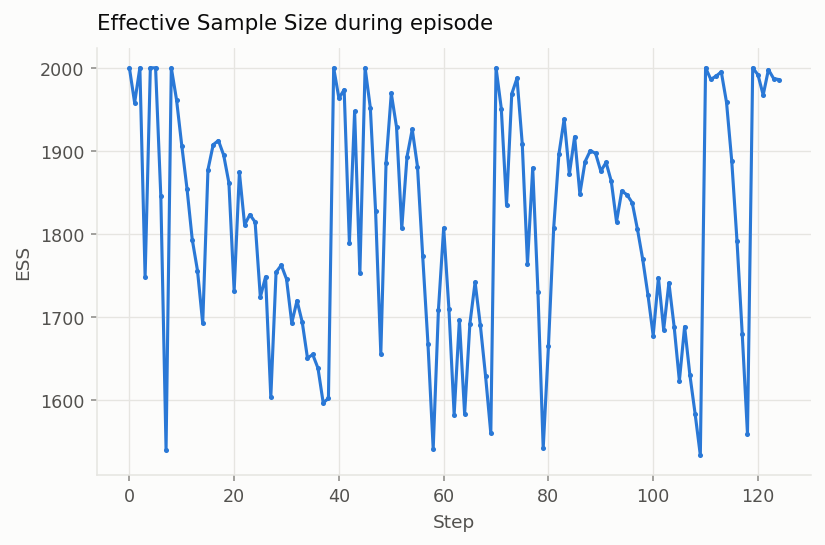
\includegraphics[width=\textwidth]{cem_ess}
    \caption{CEM}
    \label{fig:effective-sample-size-cem}
  \end{subfigure}
  \caption{Effective sample size.}
  \label{fig:effective-sample-size}
\end{figure}
ESS stays high ($\sim$1900--1960 of 2000) for both, sawtoothing against the $0.75N = 1500$ resample trigger. The particle filter is healthy; it is not the bottleneck.

\FloatBarrier
\subsection{A caveat on the baseline table}\label{sec:a-caveat-on-the-earlier-baseline-table}
The \hyperref[sec:baseline-results]{baseline results} table was produced with the batched Torch harness --- \textbf{not} the NumPy reference path. Cross-checking the two on the same model and the same $\omega$ exposed a defect in the batched harness:

\begin{table}[H]
  \centering
  \caption{A caveat on the earlier baseline table.}
  \label{tab:a-caveat-on-the-earlier-baseline-table}
  \footnotesize
  \begin{tabular}{lllll}
  \toprule
  harness & mean & median & max & episodes diverging (>1e-2) \\
  \midrule
  \texttt{rollout\_\allowbreak{}sb3} (NumPy, float64) & 2.18e-03 & 1.97e-03 & 7.7e-03 & \textbf{0 of 1000} \\
  \texttt{rollout\_\allowbreak{}generic} (Torch, float32) & 6.9e-03 & 2.31e-03 & 4.8e-01 & \textbf{5--8\%} \\
  \bottomrule
  \end{tabular}
\end{table}
In the failing episodes the particle cloud migrates onto a phase alias outside the prior support (final range e.g. \texttt{[0.\allowbreak{}34, 1.\allowbreak{}55]}, 99\% of particles outside $[0,1]$) and the posterior variance ends up \emph{larger} than the prior's --- which is impossible for a correct filter.

What has been established: the two filters agree to within 20\% when fed identical $(t, d)$ sequences, so the update and resampling code is equivalent; batching is \textbf{not} the cause (B=1 with independent seeds diverges at the same rate as B=128); and moving the batched path to float64 halves the divergence rate (4.7\% $\rightarrow$ 2.0\%) without eliminating it. The root cause is not yet pinned down.

\textbf{Consequence:} the \emph{median} column of the baseline table is sound --- the two harnesses agree there --- but the \emph{mean} column is inflated for every method that drives $t$ into the aliasing regime. Treat the medians as the ranking and regard the means as upper bounds pending a re-run through the NumPy path. Until this is fixed, the reference harness is the one to use for any number that matters.

\FloatBarrier
\subsection{Divergences from Fiderer et al.}\label{sec:divergences-from-fiderer-et-al}
The equations in this implementation match the paper. The \emph{setup} around them does not, in several places. These are documented rather than fixed, because changing any of them invalidates the shipped checkpoint and the results above; they belong in a separate, deliberate change.

\begin{center}
\footnotesize
\begin{longtable}{>{\raggedright\arraybackslash}p{0.207\linewidth}>{\raggedright\arraybackslash}p{0.268\linewidth}>{\raggedright\arraybackslash}p{0.430\linewidth}}
\caption{Divergences from Fiderer et al.}\label{tab:divergences-from-fiderer-et-al}\\
\toprule
 & Fiderer & this repo \\
\midrule
\endfirsthead
\caption[]{Divergences from Fiderer et al.\ (continued)}\\
\toprule
 & Fiderer & this repo \\
\midrule
\endhead
\bottomrule
\endfoot
discount factor $\gamma$ & \textbf{1} (required by Eq. 3) & \texttt{0.\allowbreak{}99} --- \hyperref[sec:4-gamma--099-breaks-the-bayes-risk-identity]{gotcha 4} \\
observation & mean, covariance, $\leq$30 past actions, \textbf{+ spent resource} & mean, var, 30 past actions --- \hyperref[sec:3-the-observation-is-missing-the-resource-counter-and-is-badly-scaled]{gotcha 3} \\
TRPO initialisation & imitation pretraining, then RL & from scratch (see below) \\
resource regimes & time-limited \textbf{and} experiment-limited & experiment-limited only (see below) \\
particles ($\omega$ with finite $T_2$) & $2\times10^4$ & $10^4$ train, $2\times10^3$ eval \\
TRPO hidden layers & 2 $\times$ 64 & \texttt{[256, 256]} \\
CEM hidden layer & 16, \textbf{ReLU} & 16, \textbf{Tanh} (\texttt{models/\allowbreak{}nn.\allowbreak{}py:\allowbreak{}91}) \\
CEM sampling covariance & $1/2$ & \texttt{CEM\_\allowbreak{}INIT\_\allowbreak{}STD = 1.\allowbreak{}0} \\
exp-sparse heuristic & $t_k = (9/8)^k$ & \texttt{ExponentialSweepPolicy(t0=0.\allowbreak{}1, r=1.\allowbreak{}05)} \\
bound on $t$ & none & \texttt{T\_\allowbreak{}MAX = 3000} \\
\end{longtable}
\end{center}

\subsubsection{No imitation pretraining --- the leading hypothesis for the gap}\label{sec:no-imitation-pretraining--the-leading-hypothesis-for-the-gap}
Fiderer trains in \textbf{two stages}: the network is first initialised by imitation learning on an existing heuristic ($\sigma^{-1}$, PGH, or a CEM-trained network), and only then refined with TRPO. The paper is candid that this is a stability measure --- ``this pretraining step is not strictly necessary but speeds up the training and makes RL more stable'' --- and every TRPO curve in the paper's Fig. 2 is pretrained, with the seed heuristic named in the legend.

\textbf{This implementation trains TRPO from scratch.} Given that the resulting policy is unstable (35.6\% of actions on the action floor) and loses to a constant on 99.85\% of frequencies, this is the single most likely explanation for the gap, ahead of the $\gamma$ bug. It is also the largest piece of missing machinery: a behaviour-cloning stage feeding into TRPO.

\subsubsection{Only the experiment-limited regime is implemented}\label{sec:only-the-experiment-limited-regime-is-implemented}
The paper studies two kinds of episode: \textbf{experiment-limited} (a fixed number $N$ of measurements) and \textbf{time-limited} (a fixed budget of total evolution time $T$, so cheap short measurements buy more shots). Only the former is implemented here.

That matters for expectations: the paper's headline claim --- an improvement over PGH of ``more than one order of magnitude'' --- is specifically for \textbf{time-limited $\omega$ estimation with $T_2 = 10$}. \textbf{That result cannot be reproduced here}, because there is no time-limited environment. In the experiment-limited panels the reported NN advantage over PGH is considerably more modest.

\subsubsection{What is \emph{not} the explanation: particle count}\label{sec:what-is-not-the-explanation-particle-count}
Evaluation uses $2\times10^3$ particles where the paper uses $2\times10^4$ for exactly this finite-$T_2$ case, which looked like a plausible reason for the adaptive heuristics doing poorly --- a depleted filter losing the fringe as $t$ grows. \textbf{Measured, and it is not.} At 512 $\omega$, seed 42:

\begin{table}[H]
  \centering
  \caption{What is \emph{not} the explanation: particle count.}
  \label{tab:what-is-not-the-explanation-particle-count}
  \begin{tabular}{lll}
  \toprule
  heuristic & \num{2000} particles & \num{20000} particles \\
  \midrule
  PGH & 5.47e-03 & 5.32e-03 \\
  $1/\sigma$ & 8.34e-03 & 9.22e-03 \\
  \bottomrule
  \end{tabular}
\end{table}
A 10$\times$ increase moves PGH by 3\% and makes $1/\sigma$ marginally worse. Particle depletion is ruled out.

The likelier mechanism is a self-reinforcing aliasing trap. Both heuristics set $t \approx 1/\sigma$; at the variance they plateau near, that is $t \approx 11$, which is past the $t > 2\pi$ aliasing threshold for this prior. The posterior then stays multimodal, $\sigma$ stays large, $t$ stays $\approx 11$, and the heuristic cannot escape. Capping the time breaks the loop, which is exactly what the results show: PGH capped at 2 reaches 2.04e-03 against 5.19e-03 uncapped. Both heuristics are asymptotically optimal for $T_2 = \infty$, where no such threshold exists.

\FloatBarrier
\subsection{Defects that bear on the numbers}\label{sec:defects-that-bear-on-the-numbers}
The following are real and worth reading before trusting any number reported above.

\subsubsection{The action range is 300\texorpdfstring{$\times$}{x} the coherence time}\label{sec:2-the-action-range-is-300-the-coherence-time}
$t_{\max} = 3000$ with $T_2 = 10$ means $e^{-t/T_2} = e^{-300}$, which underflows to exactly \texttt{0.\allowbreak{}0} in floating point. Any $t \gtrsim 200$ yields $p_0 = 0.5$ identically --- a measurement with \textbf{literally zero} Fisher information. More than 99\% of the action range is physically useless, which makes exploration far harder than it needs to be.

This bound is an implementation choice, not the paper's: Fiderer imposes no upper limit on $t$ (its $\sigma^{-1}$ and PGH heuristics grow without one, and the exp-sparse heuristic grows geometrically forever). A bounded \texttt{Box} action space is a reasonable concession to RL, but $O(10\text{--}100)$ would cover everything physically useful. Changing it invalidates comparison with the existing checkpoints.

\subsubsection{The observation is missing the resource counter, and is badly scaled}\label{sec:3-the-observation-is-missing-the-resource-counter-and-is-badly-scaled}
Two separate problems.

\textbf{Missing input.} Fiderer specifies the observation as $\mathbb{E}[\theta \mid D_k]$, $\mathrm{Cov}(\theta \mid D_k)$, the previous actions (at most 30), \textbf{and the spent time or number of experiments in the current episode}. This implementation builds \texttt{[mean, var, *t\_\allowbreak{}history]} and omits the resource term entirely. The policy therefore cannot distinguish measurement 5 from measurement 120, which makes any correct endgame behaviour unlearnable --- there is no input that tells it the episode is ending. Fixing this means \texttt{shape=(3 + history\_\allowbreak{}size,)} and a retrain.

\textbf{Bad scaling.} What is there mixes a variance of order $10^{-4}$ with interrogation times of order $10^3$, fed unnormalised into the MLP. There is no \texttt{VecNormalize} and no \texttt{check\_\allowbreak{}env} call.

\subsubsection{\texorpdfstring{$\gamma = 0.99$}{gamma = 0.99} breaks the Bayes-risk identity}\label{sec:4-gamma--099-breaks-the-bayes-risk-identity}
Training sets \texttt{GAMMA = 0.\allowbreak{}99}. The paper sets it to \textbf{one}, and that is not incidental --- it is what makes the whole training objective correct. Fiderer Eq. (3) holds only for an undiscounted return:

\begin{equation}
\mathbb{E}_{D_N}\left[\sum_{j=1}^{N} R(D_j)\right] = \mathrm{const} - r\bigl(h \mid p(\theta)\bigr).
\label{eq:undiscounted}
\end{equation}
``RL has the goal to maximize the expected discounted reward which equals the left-hand side of Eq. (3) because we set the discount factor to one.''

With $\gamma = 0.99$ over a 100-step episode, $0.99^{100} \approx 0.37$: late measurements are discounted by nearly two thirds. TRPO is then \textbf{not minimising the Bayes risk} --- it is minimising a discounted surrogate that overweights early variance reduction. Combined with the fact that the posterior variance collapses by two orders of magnitude within the first $\sim$20 measurements (so per-step rewards after that are $\sim 10^{-5}$ regardless), the late-episode signal is close to nonexistent.

\textbf{Setting $\gamma = 1$ is a precondition for drawing any conclusion about the method.} This is the most likely cause of the greedy, unstable behaviour in the \hyperref[sec:baseline-results]{baseline results} --- 35.6\% of actions pinned to the $t = 0.1$ floor.

For the avoidance of doubt: the linear $\Delta V$ reward is not itself the defect, and the claim that the literature uses $-\log V$ instead is wrong. The reward matches Fiderer Eq. (2) exactly and is well justified. The discount factor is the actual bug.

\subsubsection{The best result on record is unreproducible}\label{sec:7-the-best-result-in-the-repo-is-unreproducible}
Run \texttt{16eda430\ldots{}} trained for 67.9 hours, reached \texttt{mean\_\allowbreak{}final\_\allowbreak{}var} = 9.28e-4, and ended \texttt{FAILED} before its single end-of-training save. Its metric history and posterior plots survive; \textbf{its weights do not.} The best loadable policy (\texttt{caaabcb8\ldots{}}, 1000 episodes) reaches $\sim$2.85e-3, roughly 3$\times$ worse. Closing that gap requires a retrain. Periodic checkpointing has since been added so this cannot recur.

\FloatBarrier
\section{Summary}\label{sec:summary}
The physics and the estimation machinery are in place and behave: the likelihood, the Bayes-risk figure of merit, the variance-reduction reward and its telescoping identity all match the paper equation by equation, and the particle filter is healthy --- ESS stays at $\sim$1900--1960 of 2000 and is not the bottleneck. What does not hold up is the learned heuristic.

Trained TRPO and CEM policies land in a statistical tie over \num{10000} held-out frequencies, at 2.173e-03 and 2.137e-03 Bayes risk respectively. Both are beaten by doing nothing adaptive at all: a constant $t = 1$ reaches a \textbf{4.7$\times$ lower} median final posterior variance than the trained policy and wins on 99.85\% of individual $\omega$ values. This is measured, not conjectured. Until that gap is closed, no claim that the learned heuristic is doing something useful is supportable.

The candidate causes, in order of suspicion, are all \hyperref[sec:divergences-from-fiderer-et-al]{divergences from the paper} rather than anything intrinsic to the method: no imitation pretraining, $\gamma = 0.99$ instead of 1, and no resource counter in the observation. Two further qualifications limit how much weight the comparison can carry. The learned side is represented by the best \emph{loadable} checkpoint, which trained for 1000 episodes, while the 68-hour run scored 3$\times$ better before losing its weights; and the baseline table's mean column is inflated by a defect in the batched evaluation harness, so the medians are the ranking and the means are upper bounds.

\FloatBarrier
\section{Literature}\label{sec:literature}

\end{document}
